\subsection{Katalog S.9}



a) Um das Ersatzschaltbild zu berechnen, müssen 2 Grössen berechnet werden: \\
1) Innenwiderstand \\
2) Leerlaufspannung oder Kurzschlussstrom \\
\\
1) Für die Berechnung des Innenwiderstandes werden alle Quellen zu null Gesetzt. \\
D.h. Spannungsquellen $\rightarrow$ Kurzschluss, Stromquellen $\rightarrow$ Leerlauf \\
\textbf{Ersatzschaltbild}


\begin{center}
  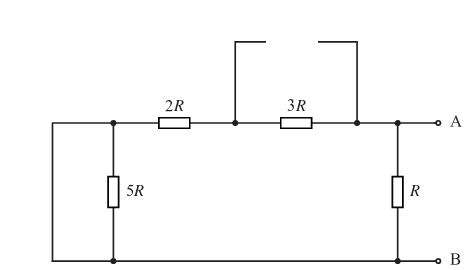
\includegraphics[scale=1.5]{katalog/katalog-1/ir-1.png} \\
\end{center}
Da der 5R Widerstand kurzgeschlossen ist, wird niemals Strom durch ihn hindurchfliessen. Somit können wir ihn durch einen Leerlauf ersetzen. \\
\begin{center}
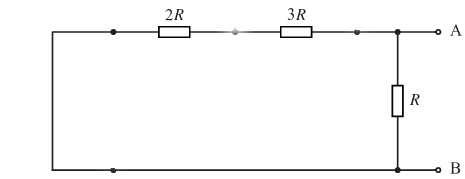
\includegraphics[scale=1.5]{katalog/katalog-1/ir-2.png} \\
\end{center}

2R und 3R liegen Seriell, somit können sie zu einem Widerstand der Grösse 5R zusammengefasst werden. \\
Dieser Widerstand ist wiederum parallel zu R, womit wir für den gesamten Widerstand und somit $R_E$ folgendes erhalten. \\
\begin{center}
  $R_E = (2R + 3R || R) = \frac{5R^2}{6R} = \frac{5}{6}R$
\end{center}

2) Nun müssen wir noch die Leerlaufspannung der Ersatzschaltung berechnen. Dazu wenden wir das Superpositionsprinzip an: \\
Zuerst berechnen wir die Spannung $U_{AB}$ zwischen den Klemmen A und B in Abhängigkeit der Spannungsquelle: \\


\begin{center}
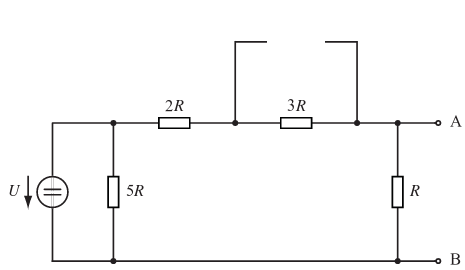
\includegraphics[scale=1.5]{katalog/katalog-1/uu-1.png}

\end{center}
\newpage
Die Widerstände 2R und 3R sind seriell.
\begin{center}
    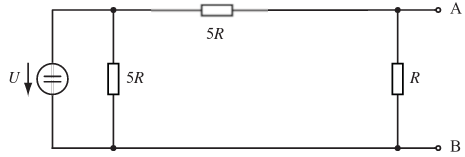
\includegraphics[scale=1.5]{katalog/katalog-1/uu-2.png}
\end{center}

Da die Widerstandände ($ 5R + R$ und $5R$) parallel sind, muss über beiden Ästen die Gleiche Spannung U abfallen. \\
Somit können wir die Spannungsteilerregel anwenden: \\
\begin{center}
    $U_{AB}^{(1)} = U \cdot \frac{R}{R + 5R} = U \cdot \frac{1}{6}$
\end{center}

Nun müssen wir noch die Spannung $U_{AB}^{(2)}$ in Abhängigkeit der Stromquelle berechnen: \\
Dazu setzen wir die Spannungsquelle zu 0:
\begin{center}
  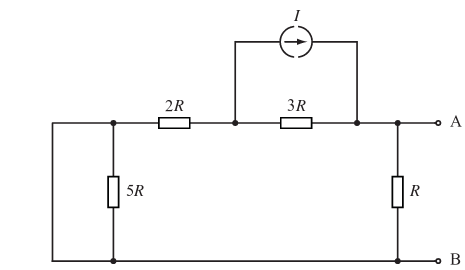
\includegraphics[scale=1.5]{katalog/katalog-1/iu-1.png}
\end{center}
Der Widerstand $R_5$ wird wieder kurzgeschlossen.
\begin{center}
  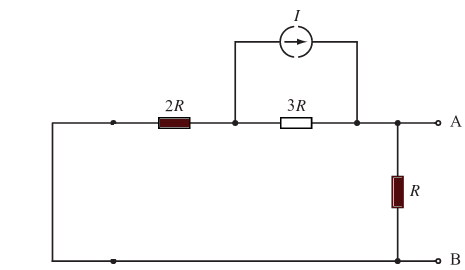
\includegraphics[scale=1.5]{katalog/katalog-1/iu-2.png}
\end{center}
Die Widerstäde $2R$ und $R$ können Seriell zusammengefasst werden, wodurch jedoch die Klemmen verschwinden :
\begin{center}
  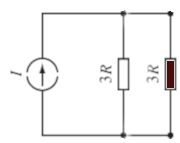
\includegraphics[scale=2.0]{katalog/katalog-1/iu-3.png} \\
\end{center}

Nun können wir mithilfe der Stromteilerregel den Strom durch den roten Widerstand berechnen:
\begin{center}
  $I_{Rot} = I \frac{3R}{3R + 3R} = \frac{I}{2}$
\end{center}

Dieser Strom fliesst durch die beiden Widerstände $R$ und $2R$ somit gilt für die Spannung über dem roten $R$ Widerstand und somit für die Spannung $U_{AB}^{(2)}$:
\begin{center}
  $U_{AB}^{(2)}  = U_R = I_{Rot}\cdot R = \frac{I\cdot R}{2}$
\end{center}

\newpage
Somit gilt für die Leerlaufspannung gemäss Superposition:
\begin{center}
  $U_{E} = U_{AB}^{(1)} + U_{AB}^{(2)} = \frac{U}{6} + \frac{I\cdot R}{2}$
\end{center}


b) Es gilt: $R_E = \frac{5}{6} \cdot 12 \Omega = 10\Omega$ und $U_E = 2V + 3A\cdot 6\Omega = 20V$ \\
Für $I_E$ gilt:
\begin{center}
  $I_E = \frac{U_E}{R_E} = \frac{20V}{10\Omega} = 2A$
\end{center}


c) Um die Leistung über dem Widerstand $R_2$ zu maximiere, schliessen wir zuerst das Lastnetzwerk an unsere Ersatzquelle an und ersetzen danach den Widerstand $R_2$ mit offenen Klemmen und Formen erneut das Netzwerk zu einer realen Quelle um. Aus der Vorlesung ist bekannt, dass die Leistung über $R_2$ genau dann maximal ist, wenn $R_2 = R_i$ gilt, wobei $R_i$ den Innenwiderstand gegenüber den Klemmen bezeichnet. \\
Die Aufgabe reduziert sich als darauf, den Innenwiderstand gegenüber den Klemmen zu berechnen.
\begin{center}
        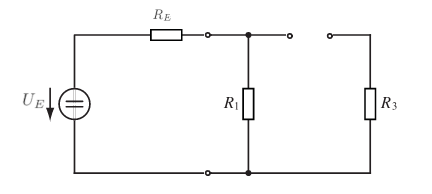
\includegraphics[scale=2.0]{katalog/katalog-1/lr-2.png}
        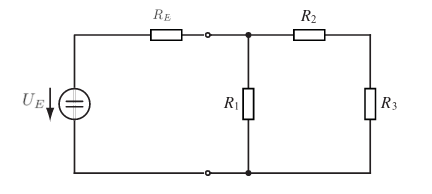
\includegraphics[scale=2.0]{katalog/katalog-1/lr-1.png}
\end{center}

Um den Innenwiderstand zu berechnen setzen wir die Quellen zu 0 und formen das Netzwerk um, bis nur noch ein Widerstand vorhanden ist. \\
\begin{center}

      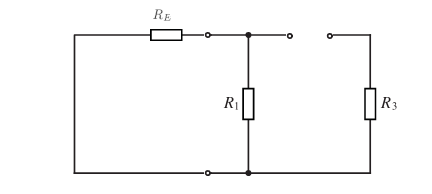
\includegraphics[scale=2.0]{katalog/katalog-1/lr-3.png}
\end{center}
Im ESB sind die Widerstände $R_E$ und $R_1$ parallel. Beide zusammen sind wiederum seriell zu $R_3$. Somit gilt für den Innenwiderstand: \\
$R_i = (R_E || R_1) + R_3$ \\
Um maximale Leistung an $R_2$ abzugeben, muss folgendes gelten:
\begin{center}
  $R_2 = R_i = (R_E || R_1) + R_3 \Rightarrow R_3 = R_2 - (R_E || R_1)$ \\
  $R_3 = 11.5 \Omega - (5\Omega || 20 \Omega) = 7.5 \Omega$
\end{center}

\newpage
d) Um den Spannungsabfall über $R_2$ zu berechnen, berechnen wir die Leerlaufspannung an den Klemmen:
\begin{center}
        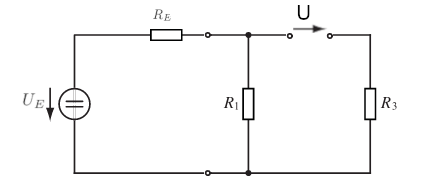
\includegraphics[scale=2.0]{katalog/katalog-1/lr-4.png} \\
\end{center}

Da durch den Widerstand $R_3$ kein Strom fliesst, gilt für die Spannung $U$:
\begin{center}
  $ U = U_{R_1} - U_{R_3} = U_{R_1} - 0A \cdot R_3 = U_{R_1}$
\end{center}
Die Spannung über $R_1$ können wir mithilfe des Spannungsteilers berechnen: \\
\begin{center}
  $U_{R_1} = U_E \cdot \frac{R_1}{R_E + R_1} = 15V \cdot \frac{20\Omega}{25\Omega} = 12V$
\end{center}
Aus der Vorlesung ist bekannt, dass bei maximaler Leistungabgabe, die Spannung über dem Lastwiderstand gerade die hälfte der Leerlaufspannung beträgt. Somit gilt für die Spannung über $R_2$:
\begin{center}
  $U_2 = \frac{U}{2} = 6V $ \\
  $P_2 = \frac{U_2^2}{R_2} = \frac{36V^2}{11.5\Omega} = 3.13W$
\end{center}





\newpage



\subsection{Katalog S.15}


\begin{itemize}
  \item a) Da es sich beim Spannungsmessgerät um ein Messgerät mit unendlich hohem Widerstand handelt, dürfen wir davon ausgehen, dass zwischen den Klemmen A und B kein Strom fliessen kann. Somit können wir die Verbindung zwischen A und B als Leerlauf modelieren.
  \begin{center}
      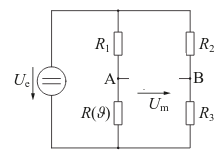
\includegraphics[scale=2.5]{katalog/katalog-1/a2-1.png}
  \end{center}
  Da die beiden Widerstandsäste parallel gescchaltet sind, muss über beiden Ästen die gleiche Spannung abfallen:
  \begin{center}
    $U_e = U_{R_1} + U_{R_\vartheta} = U_{R_2} +U_{R_3}$
  \end{center}
  Somit können wir die Spannung über $R_\vartheta$ mithilfe des Spannungsteilers berechnen:
  \begin{center}
      $U_{R_\vartheta} = U_e \cdot \frac{R_\vartheta}{R_1 + R_\vartheta}$
  \end{center}
  Die Leistung über einem Widerstand ist definiert als:
  \begin{center}
    $P_R = U_R \cdot I_R = \frac{U_R^2}{R}$
  \end{center}
  Somit gilt für die Leistung über dem Widerstand $R_\vartheta$ ;
  \begin{center}
      $P_{R_\vartheta} = \frac{U_{R_\vartheta}^2}{R_\vartheta} = (U_e \cdot \frac{R_\vartheta}{R_1 + R_\vartheta})^2 \cdot \frac{1}{R_\vartheta} =  \frac{U_e^2 \cdot R_\vartheta}{(R_1 + R_\vartheta)^2} $
  \end{center}

  Um den Maximalwert dieser Leistung in Abhängigkeit des Widerstandes $R_\vartheta$ herauszufinden, leiten wir die Leistung nach $R_\vartheta$ ab und setzen sie zu 0:
  \begin{center}
    $\frac{d}{dR_\vartheta}(P_{R_\vartheta}) \stackrel{!}{=} 0 \rightarrow R_\vartheta = R_1 = 1k \Omega$
  \end{center}
  Die benötigte Temperatur berechnet sich zu:
  \begin{center}
    $R(\vartheta) = 1k\Omega (1 + \alpha (\vartheta - \vartheta_0)) \stackrel{!}{=} 1k \Omega$ \\
    $\Rightarrow \vartheta = \vartheta_0 = 20$\textdegree
  \end{center}
  Für die Spannung $U_e$ erhalten wir:
  \begin{center}
    $50mW \stackrel{!}{=} P_{R_\vartheta} = U_e^2 \cdot \frac{1k\Omega}{4k\Omega}$ \\
    $\rightarrow 200mW = U_e^2$ \\
    $ \rightarrow U_e = 14.14V$
  \end{center}
  \item b) Für die Spannung $U_m$ können wir folgende Masche aufstellen:
  \begin{center}
    $U_m = U_{R_\vartheta} - U_{R_3}$
  \end{center}
  Wobei wir $ U_{R_\vartheta}$ und $U_{R_3} $ mit dem Spannungsteiler berechnen können:
  \begin{center}
    $U_{R_\vartheta} = U_e \frac{R_\vartheta}{R_\vartheta + R_1} $ \\
      $U_{R_3} = U_e \frac{R_3}{R_2 + R_3} $
  \end{center}
  Somit gilt für $U_m$:
  \begin{center}
    $U_m = U_e \big(\frac{R_\vartheta}{R_\vartheta + R_1}  - \frac{R_3}{R_2 + R_3} \big)$
  \end{center}
  Mit der Bedingung, $U_m(\vartheta = \vartheta_0 = 0 $\textdegree$) = 0V$ erhalten wir:

  \begin{center}
      $0V= U_e \big(\frac{R(\vartheta_0 )}{R(\vartheta_0) + R_1}  - \frac{R_3}{R_2 + R_3} \big) = U_e \big(\frac{0.9 k\Omega}{1.9 k\Omega}  - \frac{R_3}{R_2 + R_3} \big)$ \\
      $\rightarrow \frac{R_3}{R_2 + R_3} = \frac{0.9 k\Omega}{1.9 k\Omega}  $ \\
      $\rightarrow R_3 = \frac{0.9}{1.9} \cdot (R_2 + R_3) $
  \end{center}

  Für die Leistung gilt:
  \begin{center}
    $P_{(R_2,R_3)} = \frac{U_e^2}{R_2 + R_3}  \stackrel{!}{=} 10mW$ \\
    $\rightarrow (R_2 + R_3) = \frac{U_e^2}{10mW} = 14400\Omega$
  \end{center}
  Somit gilt:
  \begin{center}
    $R_3 = \frac{0.9 k\Omega}{1.9 k\Omega} \cdot (14400\Omega) = 6821.05 \Omega $ \\
    $R_2 = 14400\Omega - R_3 = 7578.95 \Omega$
  \end{center}


  \item c) Wir bezeichnen mit $U_{ideal}$ die Spannung bei idealer Messung und mit $U_{err}$ die Spannung mit ungenauen Widerständen.
  \begin{center}
    $U_{ideal} = 12V \big( \frac{R_\vartheta}{R_\vartheta + R_1} - \frac{R_3}{R_3 + R_2}\big)$ \\
    $U_{err} = 12V \big( \frac{R_\vartheta}{R_\vartheta + R_1' } - \frac{R_3'}{R_3'+R_2'}\big)$
  \end{center}
  Die Differenz ist:
  \begin{center}
    $F(R_\vartheta)) = U_{ideal} - U_{err} = U_e \big (\frac{R_\vartheta}{R_\vartheta + R_1 } -\frac{R_\vartheta}{R_\vartheta + R_1'} - \frac{R_3}{R_3 + R_2} + \frac{R_3'}{R_3'+R_2'})$
  \end{center}
  Der Fehler wird maximal, wenn die Differenz stark negativ wird. Dies ist der Fall, falls $\frac{R_3'}{R_3'+R_2'} < \frac{R_3}{R_3+R_2}$ und $  \frac{R_\vartheta}{R_\vartheta + R_1'} > \frac{R_\vartheta}{R_\vartheta + R_1}$  gilt. Somt gilt für die Widerstände:

   \begin{center}
     $R_3' < R_3 \rightarrow R_3' = 0.9 \cdot R_3$ \\
      $R_2' > R_2 \rightarrow R_2' = 1.1 \cdot R_2$ \\
      $R_1' < R_1 \rightarrow R_1' = 0.9 \cdot R_1$
   \end{center}
  Um die Temperatur herauszufinden, leiten wir die Differenz nach $R_\vartheta$ ab:
  \begin{center}
    $\frac{d}{d R_\vartheta} (F(R_\vartheta)) \stackrel{TR}{=} U_e \cdot \big( \frac{R_1}{(R_1 + R_\vartheta)^2} - \frac{R_1'}{(R_1' + R_\vartheta)^2}\big)\stackrel{!}{=} 0$ \\
    $\stackrel{TR}{\rightarrow} R_\vartheta = \sqrt{R_1 \cdot R_1'} = 0.949 \cdot R_1 = 949 \Omega$ \\
    $\rightarrow (1 + \alpha (\vartheta - \vartheta_0)) = 0.949  $ \\
    $\rightarrow \vartheta = 9.8$\textdegree
  \end{center}
  Der Betrag des Fehler berechnet sich zu:
  \begin{center}
      $ U_{err} = 12V \big( \frac{R_\vartheta}{R_\vartheta + R_1'} - \frac{R_3'}{R_3' + R_2'} \big) = 1.07V$ \\
      $ U_{ideal} \stackrel{!}{=} 1.07V \rightarrow R_\vartheta = $
  \end{center}
\end{itemize}

\newpage

\subsection{Katalog S. ???}



a) Es gilt:
 \begin{center}
  $\iint _A \vec{J}(\vec{r}) \cdot d\vec{A} = I$.
\end{center}
Falls das J-Feld und die Fläche \textbf{senkrecht} sind und das J-Feld überall auf dieser Fläche  \textbf{gleich Gross} ist, vereinfacht sich dies zu:
\begin{center}
  $ A_{eff}(\vec{r}) \cdot J(\vec{r})  = I \Rightarrow J(\vec{r}) = \frac{I}{A_{eff}(\vec{r})}$ \\
\end{center}
Wobei $A_{eff}$ die effektiv vom Strom durchflossene Fläche bezeichnet.
\end{itemize}
Somit gilt für die Stromdichte im Messwiderstand:
\begin{center}
  $ J(r) = \frac{I}{d \cdot 2 \pi r}$ \\
\end{center}

und somit in Vektorform (Zylinderkoordinaten):
\begin{center}
  $ \vec{J}(r) = \frac{I}{d \cdot 2 \pi r} \cdot \vec{e}_{r}$ \\
\end{center}

\item b) Der Zusammenhang zwischen E-Feld und J-Feld ist gegeben als:
\begin{center}
  $\vec{E} = \frac{1}{\kappa} \cdot \vec{J}$
\end{center}
Somt gilt für das E-Feld:
\begin{center}
    $\vec{E}(r) =  \frac{I}{d \cdot 2 \pi r \cdot \kappa} \cdot \vec{e}_{r}$
\end{center}
Für die Spannung $U_{AB}$ gilt: \\
\begin{center}
  $U_{AB} = \int_A^B \vec{E}(r) \cdot d\vec{s} = \int_{\frac{D_{Innen}}{2}}^{\frac{D_{Aussen}}{2}} E(r) \cdot dr =  \int_{\frac{D_{Innen}}{2}}^{\frac{D_{Aussen}}{2}} \frac{I}{d \cdot 2 \pi r \cdot \kappa} \cdot dr = \underline{\underline{\frac{I}{\kappa \cdot d \cdot 2 \pi} \cdot ln(\frac{D_{aussen}}{D_{innen}})}}$
\end{center}
Für den Widerstand R gilt:
\begin{center}
$  R_{AB} := \frac{U_{AB}}{I} = \frac{1}{\kappa \cdot d \cdot 2 \pi} \cdot ln(\frac{D_{aussen}}{D_{innen}})$
\end{center}

Mit den Werten: $D_{aussen} = 2cm$, $D_{innen} = 5mm$ , $d = 3mm$ und $\kappa = 12 \cdot 10^3 \frac{S}{m}$ gilt:
\begin{center}
  $R_{AB} = \frac{1}{12 \cdot 10^3 \frac{S}{m} \cdot 3\cdot 10^{-3} m \cdot 2 \pi} \cdot ln(\frac{2 \cdot 10^{-2}}{3 \cdot 10^{-3}}) = 8.387m\Omega$
\end{center}
\item c) Wir betrachten beide Fälle (-3mm und +3mm):  \\
 +3mm: $\rightarrow R' = \frac{1}{12 \cdot 10^3 \frac{S}{m} \cdot 3\cdot 10^{-3} m \cdot 2 \pi} \cdot ln(\frac{2 \cdot 10^{-2} + 3 \cdot 10^{-3}}{3 \cdot 10^{-3}}) = 9.005m\Omega \rightarrow \Delta R =  |R-R'| = 0.618 m\Omega$\\
 -3mm: $\rightarrow R' = \frac{1}{12 \cdot 10^3 \frac{S}{m} \cdot 3\cdot 10^{-3} m \cdot 2 \pi} \cdot ln(\frac{2 \cdot 10^{-2} - 3 \cdot 10^{-3}}{3 \cdot 10^{-3}}) = 7.669m\Omega \rightarrow \Delta R =  |R-R'| = 1.336 m\Omega$\\
 Daraus Folgt: Maximaler Fehler bei $-3mm$. $R'$ ist dann $7.669m\Omega$ und für den Fehler gilt: $ \Delta R = 1.336 m\Omega$
\end{center}


\item d) Beim Messen gilt:
\begin{center}
 $\frac{U_{AB}}{R_{AB}} = I \rightarrow \Delta I =  |\frac{U_{AB}}{R_{AB}} - \frac{U_{AB}}{R'_{AB}} | $ \\
 $ F = \frac {\Delta I}{I} = \frac{\Delta I}{U_{AB}/R_{AB}} = |1 - \frac{R_{AB}}{R'_{AB}}| = |1 - \frac{8.387m\Omega}{ 7.669}| = 9.28\% $
\end{center}


\item e) es gilt: $ U_{AC} = \int_{r_a}^{r_c} E \cdot dr$ und  $ U_{CB} = \int_{r_c}^{r_b} E \cdot dr$.  \\
Das Integral $\int_{r_a}^{r_b} E \cdot dr$ haben wir bereits ausgerechnet. Es ergibt:
$ \frac{I}{\kappa \cdot d \cdot 2 \pi} \cdot ln(\frac{r_b}{r_a}) $ \\
Somit lautet die Gleichung:
\begin{center}
  $ \frac{I}{\kappa \cdot d \cdot 2 \pi} \cdot ln(\frac{r_c}{\frac{D_{innen}}{2} }) = \frac{I}{\kappa \cdot d \cdot 2 \pi} \cdot ln(\frac{\frac{D_{aussen}}{2}}{r_c })$ \\
  $ \Rightarrow \frac{2 r_c}{D_{innen}} = \frac{D_{aussen}}{2 r_c} \rightarrow r_c = \frac{\sqrt{D_{aussen} \cdot D_{innen}}}{2} = 5mm$
\end{center}
